\chapter{Ideen und Konzepte}
\label{ch:Ideen_und_Konzepte}

\section{Single-User Prototyp}
Um dem Nutzer die Interaktion mit den Bauteilen so intuitiv und angenehm wie möglich zu machen, sind die folgenden Features in der Umsetzung geplant:

\subsection{Highlight}
\label{ch:highlight}
Um dem Benutzer zu zeigen, mit welchem Bauteil er interagieren kann, soll das Bauteil, in welchem sich seine Hand aktuell befindet, markiert werden. Dabei soll die Markierung für den Benutzer gut sichtbar sein, nicht aber die Sicht auf das Bauteil selbst versperren. \\
Im SteamVR-Asset befindet sich eine Beispiel Szene (Interactions\_Example), um die Handhabung mit dem Asset besser kennen zu lernen. In dieser Szene werden Objekte mit einer gelben Umrandung versehen, zu sehen in Abbildung \ref{fig:steamvr_highlight}, sobald sich ein Controller des Benutzers im Objekt befindet.

\begin{figure}[h!]
	\centering
	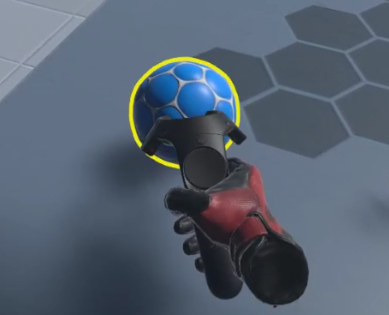
\includegraphics[keepaspectratio,width=0.4\linewidth]{img/SteamVR_Highlight.PNG}
	\caption{SteamVR Highlight}
	\label{fig:steamvr_highlight}
\end{figure}
	
\subsection{Snapping}
Bauteile in der virtuellen Realität präzise zu platzieren kann oft sehr schwierig sein. Um dem entgegenzuwirken sollen Bauteile, welche sich in der Nähe ihres vorgesehenen Ortes befinden, beim loslassen automatisch an ihre richtige Position bewegt werden. Um dem Benutzer mitzuteilen, dass das Bauteil an eine Position \grqq gesnappt\grqq{} werden kann, soll die Silhouette des Bauteils am vorgesehen Ort erscheinen. Um die Silhouette erscheinen zu lassen, könnte die gelbe Umrandung verwendet werden, welche im Kapitel \ref{ch:highlight} bereits erwähnt wurde. 
	
\subsection{Kollision}
\label{ch:kollision}
Beim Bewegen der Bauteile sollten diese mit anderen Bauteilen, welche sich in der virtuellen Umgebung befinden, kollidieren. Da alle Bauteile aber nur virtuell verfügbar sind und die Hand in der realen Welt nicht an etwas abprallen kann, muss dies in der virtuellen Realität simuliert werde. \\
Um dies zu Realisieren müssen beide Bauteile einen Collider besitzen. Sobald ein Kollisions-Event gesendet wird, wird das Bauteil von der Hand des Spielers losgelöst. Die Physik-Engine von Unity berechnet dann welche Auswirkungen die Kollision auf das Bauteil hat.
	
\subsection{Feedback beim Zusammenbau / Manipulation der Objekte}
\label{ch:feedback_zusammenbau_konzepte}
Da Bauteile nicht durch andere Bauteile hindurch bewegt werden können, muss dem Benutzer eine Art Feedback gegeben werden, sobald zwei Bauteile kollidieren. Dies soll dem Benutzer auch beim Zusammenbauen der Objekte behilflich sein. In der Tabelle \ref{tbl:varianten_zusammenbau} sind drei Varianten aufgelistet, welche dieses Problem lösen könnten. Anhand eines Nutzertests soll evaluiert werden, welcher dieser Varianten sich am besten für dieses Problem eignet.
	
\begin{center}
	\begin{tabularx} {\textwidth} { | B | B | B | }
		\hline
		\rowcolor{black}
		\color{white} \textbf{Variante} & \color{white} \textbf{Pro} & 
		\color{white} \textbf{Contra} \\
		\hline
		\vspace{1pt}
		Visuelles Feedback, falls ein Bauteil mit einem anderen kollidiert & 
		\begin{itemize} [leftmargin=*,noitemsep,topsep=0pt]
			\item Ist für alle Nutzer sichtbar
		\end{itemize} &
		\begin{itemize} [leftmargin=*,noitemsep,topsep=0pt]
			\item Kann dem Benutzer sehr unnatürlich erscheinen
		\end{itemize} \\
		\hline
		\vspace{1pt}
		Einschränkungen der Freiheitsgrade sobald das Bauteil eine gewisse Position erreicht, wie in Abbildung \ref{fig:VADEAssembly} zu sehen. 
		\vspace{2pt} & 
		\begin{itemize} [leftmargin=*,noitemsep,topsep=0pt]
			\item Das Zusammenbauen des Bauteils wird dem Benutzer erleichtert
		\end{itemize} &
		\begin{itemize} [leftmargin=*,noitemsep,topsep=0pt]
			\item Kein Feedback falls eine falsche Bewegung durchgeführt wird
		\end{itemize} \\
		\hline
		\vspace{1pt}
		Vibration Feedback bei einer falschen Bewegung & 
		\begin{itemize} [leftmargin=*,noitemsep,topsep=0pt]
			\item Der Benutzer bemerkt die falsche Bewegung, ohne hinzusehen
		\end{itemize} &
		\begin{itemize} [leftmargin=*,noitemsep,topsep=0pt]
			\item Nur der bearbeitende Benutzer bemerkt die falsche Bewegung
		\end{itemize} \\
		\hline	
	\end{tabularx}
\end{center}
\captionof{table}{Varianten für das Feedback beim Zusammenbau}\label{tbl:varianten_zusammenbau}

\subsection{Architektur}
% TODO: Architektur Diagramm

\pagebreak
\section{Multi-User Prototyp}
Der Multi-User Prototyp soll auf dem Single-User Prototyp aufbauen und alle Features von diesem implementieren. Die Erkenntnisse aus der ersten Nutzerevaluation sollen ebenfalls in den zweiten Prototypen einfliessen.

Anhand der Erkenntnissen aus den Recherchen, sind die folgenden Features in der Umsetzung geplant:

\subsection{Avatar-Repräsentation in der virtuellen Umgebung}
\label{ch:avatar_repraesentation_realisierung}
Anhand der Recherchen, siehe Kapitel \ref{ch:avatar_repraesentation}, wurden folgende Varianten für eine Avatar-Repräsentation gefunden:
\begin{center}
	\begin{tabularx} {\textwidth} { | B | B | B | }
		\hline
		\rowcolor{black}
		\color{white} \textbf{Variante} & \color{white} \textbf{Pro} & 
		\color{white} \textbf{Contra} \\
		\hline
		\vspace{1pt}
		Kopf und Hände der Benutzer werden in der virtuellen Umgebung abgebildet & 
		\begin{itemize} [leftmargin=*,noitemsep,topsep=0pt]
			\item Gesten und Gaze können dargestellt werden
		\end{itemize} & 
		\begin{itemize} [leftmargin=*,noitemsep,topsep=0pt]
			\item Den Kopf und die Hände ohne Körper zu sehen kann sehr unnatürlich wirken
		\end{itemize} \\
		\hline
		\vspace{1pt}
		Einfacher Avatar welcher den Oberkörper abbildet & 
		\begin{itemize} [leftmargin=*,noitemsep,topsep=0pt]
			\item Funktioniert ohne zusätzliche Detektoren
		\end{itemize} & 
		\begin{itemize} [leftmargin=*,noitemsep,topsep=0pt]
			\item Versperrt dem andern Benutzer möglicherweise die Sicht auf Teile von relevanten Objekten
		\end{itemize} \\
		\hline
		\vspace{1pt}
		Ganzkörper Avatar & 
		\begin{itemize} [leftmargin=*,noitemsep,topsep=0pt]
			\item Ganzkörper Repräsentation des Gegenübers, erscheint daher natürlicher
		\end{itemize} & 
		\begin{itemize} [leftmargin=*,noitemsep,topsep=0pt]
			\item Schwer umzusetzen bezüglich des Trackings, da zusätzliche Detektoren verwendet werden müssen. Falls diese nicht richtig funktionieren erscheint der Avatar dem Gegenüber unnatürlich
		\end{itemize} \\
		\hline	
	\end{tabularx}
\end{center}
\captionof{table}{Varianten für die Avatar-Repräsentation}\label{tbl:varianten_avatar}

\bigskip
Für diesen Typ Applikation ist es nicht notwendig einen Ganzkörper Avatar zu verwenden. Dieser würde nur weitere Detektoren benötigen und bringt keinen Mehrwert. Die Gesten können auch mit einem einfachen Avatar dem Gegenüber gezeigt werden. \\
\noindent Ein einfacher Avatar bestehend aus Kopf, Oberkörper und den beiden Händen kann ohne zusätzlichen Detektoren umgesetzt werden. Dabei sehen die anderen Benutzer zusätzlich die Orientierung der anderen Benutzern, was für die Zusammenarbeit von Vorteil sein kann. Dementsprechend wird im Projekt ein Avatar mit einem Oberkörper verwendet.

\subsection{Kommunikation zwischen den Benutzern}
\label{ch:kommunikation_zwischen_benutzern}

\begin{center}
	\begin{tabularx} {\textwidth} { | B | B | B | }
		\hline
		\rowcolor{black}
		\color{white} \textbf{Variante} & \color{white} \textbf{Pro} & 
		\color{white} \textbf{Contra} \\
		\hline
		\vspace{1pt}
		Audio-Aufnahmen mit dem Mikrofon und Wiedergabe über die Kopfhörer des Gerätes & 
		\begin{itemize} [leftmargin=*,noitemsep,topsep=0pt]
			\item Kann über jegliche Distanzen verwendet werden
		\end{itemize} & 
		\begin{itemize} [leftmargin=*,noitemsep,topsep=0pt]
			\item Das Gerät muss ein Mikrofon sowie ein Lautsprecher besitzen
		\end{itemize} \\
		\hline
		\vspace{1pt}
		Direkte Kommunikation mit dem Gegenüber & 
		\begin{itemize} [leftmargin=*,noitemsep,topsep=0pt]
			\item Benötigt keine technische Implementation
		\end{itemize} & 
		\begin{itemize} [leftmargin=*,noitemsep,topsep=0pt]
			\item Beide Benutzer müssen sich im selben Raum befinden
		\end{itemize} \\
		\hline
		\vspace{1pt}
		Kommunikation anhand der Körpersprache - Gesten und Gaze & 
		\begin{itemize} [leftmargin=*,noitemsep,topsep=0pt]
			\item Einfach und verständlich
		\end{itemize} & 
		\begin{itemize} [leftmargin=*,noitemsep,topsep=0pt]
			\item Eingeschränkte Kommunikation
		\end{itemize} \\
		\hline	
	\end{tabularx}
\end{center}
\captionof{table}{Varianten für die Kommunikation zwischen den Benutzern}\label{tbl:varianten_kommunikation}

\bigskip
Da die Applikation auch verteilt über mehrere Standorte funktionieren soll, muss entweder Variante eins oder drei aus der Tabelle \ref{tbl:varianten_kommunikation} umgesetzt werden.  \\
Da die HTC Hive ein Mikrophon sowie Kopfhörer integriert hat, kann die erste Variante ohne zusätzliche Hardware umgesetzt werden. Um die Kommunikation zwischen den Benutzern so verständlich wie möglich zu machen wird zusätzlich zu der ersten Variante noch die dritte Variante umgesetzt, welche dank dem geplanten Avatar, beschrieben in Kapitel \ref{ch:avatar_repraesentation_realisierung}, implementiert werden kann.


\subsection{Gleichzeitige Interaktion am selben Objekt}
\label{ch:gleichzeitige_interaktion}
Falls zwei Benutzer gleichzeitig dasselbe Objekt manipulieren wollen, muss eine Lösung gefunden werden, damit keine Inkonsistenzen zwischen den Benutzern entsteht, falls ein Benutzer das Bauteil an einen anderen Ort bewegt als der andere. Im Bereich der Gleichzeitigen Interaktion am selben Objekt gibt es sehr viele Varianten, über welche Forschungen und Paper veröffentlicht worden sind (siehe Kapitel \ref{ch:collaborative_user_interaction}). Anhand dieser wurde die nachfolgende Tabelle erstellt:

\begin{center}
	\begin{tabularx} {\textwidth} { | B | B | B | }
		\hline
		\rowcolor{black}
		\color{white} \textbf{Variante} & \color{white} \textbf{Pro} & 
		\color{white} \textbf{Contra} \\
		\hline
		\vspace{1pt}
		Separierung der Freiheitsgrade – Ein Nutzer steuert die Position, ein anderer die Rotation des Objektes &  &
		\begin{itemize} [leftmargin=*,noitemsep,topsep=0pt]
			\item Umständlich für eine Engineering Applikation
			\item Behindert die Zusammenarbeit
			\item Maximal zwei Benutzer
		\end{itemize} \\
		\hline
		\vspace{1pt}
		Berechnung des Mittelwerts aller Inputs der Nutzer & 
		\begin{itemize} [leftmargin=*,noitemsep,topsep=0pt]
			\item Gleichzeitige Manipulation
		\end{itemize} & 
		\begin{itemize} [leftmargin=*,noitemsep,topsep=0pt]
			\item Das Manipulierte Objekt verhält sich nicht natürlich und zerstört so die Immersion
		\end{itemize} \\
		\hline
		\vspace{1pt}
		Abstrahierte Objekte in der realen Welt & 
		\begin{itemize} [leftmargin=*,noitemsep,topsep=0pt]
			\item Natürliches Verhalten
			\item Natürliches Feedback bei der Manipulation
		\end{itemize} & 
		\begin{itemize} [leftmargin=*,noitemsep,topsep=0pt]
			\item Benutzer müssen sich im selben Raum befinden
			\item Objekt und Hände müssen getracked werden
		\end{itemize} \\
		\hline
		\vspace{1pt}
		Zauberstab – Nur der Benutzer mit dem Zauberstab kann das Objekt manipulieren &
		\begin{itemize} [leftmargin=*,noitemsep,topsep=0pt]
			\item Natürliches Verhalten, da nur ein Nutzer das Objekt manipuliert
		\end{itemize} &
		\begin{itemize} [leftmargin=*,noitemsep,topsep=0pt]
			\item Nur ein Benutzer kann die Umgebung bearbeiten
		\end{itemize} \\
		\hline	
		\vspace{1pt}
		«First come, First grab» Der Benutzer welcher eine Interaktion als erstes beginnt hat so lange die Macht über das Objekt bis er dieses wieder loslässt. & 
		\begin{itemize} [leftmargin=*,noitemsep,topsep=0pt]
			\item Natürliches Verhalten, da nur ein Nutzer das Objekt manipuliert
		\end{itemize} &
		\begin{itemize} [leftmargin=*,noitemsep,topsep=0pt]
			\item Nur ein Benutzer kann das Objekt bearbeiten
			\item Andere Benutzer müssen sehen, ob sie das Objekt aktuell manipulieren können oder nicht
		\end{itemize} \\
		\hline	
	\end{tabularx}
\end{center}
\captionof{table}{Varianten für gleichzeitige Interaktion am selben Objekt}\label{tbl:varianten_gleichzeitige_interaktion}

\bigskip
Die erste Variante macht in der umzusetzende Applikation die Zusammenarbeit umständlicher als es sein muss. Da ein Objekt oftmals nicht nur die Position ändern soll sondern auch die Rotation müssten bei den meisten Interaktionen mehrere Benutzer beteiligt sein. \\
Die Variante bei welcher der Mittelwert aller Inputs genommen wird, wird ebenfalls nicht umgesetzt, da sich die Bewegung des Objektes für alle beteiligten Benutzer unnatürlich anfühlen würde. \\
Die Variante mit den abstrahierten Objekte in der realen Welt würden den Benutzern das natürlichste Verhalten geben, kann aber nicht umgesetzt werden, da die Applikation auch verteilt funktionieren soll und sich die Benutzer für diese Variante im selben Raum befinden müssten. \\
Dementsprechend werden die letzten beiden Varianten implementiert und anhand von Nutzertests evaluiert, welche Variante sich für diese Applikation besser eigenen würde.

\subsection{Architektur}